\documentclass[10pt]{article}
\usepackage[utf8]{inputenc}
\usepackage{fancyhdr}
\usepackage{graphicx}
\usepackage{eurosym}
\usepackage{amsmath}
\usepackage[ngerman]{babel}
\date{\vspace{-5ex}}
\usepackage{geometry}
\geometry{a4paper, left=25mm, right=25mm}
\renewcommand{\headrulewidth}{0pt}
\fancyhead[L]{}
\fancyhead[R]{

\includegraphics[width=4cm]{images/shack.png}
}
\usepackage{hyperref}

\newdimen\longline
\longline=\textwidth\advance\longline-4cm

\def\LayoutTextField#1#2{#2} % override default in hyperref

\def\lbl#1{\hbox to 4cm{#1\dotfill\strut}}%
\def\labelline#1#2{\lbl{#1}\vbox{\hbox{\TextField[name=#1,width=#2]{\null}}\kern2pt\hrule}}

\def\q#1{\hbox to \hsize{\labelline{#1}{\longline}}\vskip1.4ex}


\pagestyle{plain}
\title{\flushleft{FESTOOL Tischfr\"ase TF 1400}}
\begin{document}
\maketitle
\thispagestyle{fancy}
\section{Schutzkleidung}
\begin{itemize}
\item \textbf{keine Handschuhe}
\item Schutzbrille
\item Gehörschutz
\item ggf. Haare zurückbinden 
\item ggf. Atemschutz 
\end{itemize}
\section{Allgemeine Sicherheitshinweise}
\begin{itemize}
\item \textbf{Immer im Gegenlauf fräsen}
\item \textbf{Bei Arbeiten mit Metall keine Absaugung verwenden! Brandgefahr!}
\item Netzkabel aus dem Eingriffsbereich des Fräsers halten
\item Werkzeug fest einspannen - dazu Schlüssel aus der Maschinenkiste verwenden
\item Korrekte Drehzahl für jeweiliges Werkzeug und Werkstück vorwählen siehe Einstellungen 
\item Keine defekten, rissigen, verbogenen oder stumpfen Werkzeuge verwenden
\item Vor Werkzeugwechsel Maschine vom Stromnetz trennen, z.B. Stecker ziehen
\item Nach dem Fräsen von Alu Maschine gründlichst reinigen und aussaugen
\end{itemize}

\section{Inbetriebnahme}
\begin{enumerate}
\item Modul in CMS Tisch einsetzen
\item Modul verriegeln
\item Strom an CMS anschliessen
\item Netzstecker des CMS an Staubsauger anschliessen
\item Staubsauger auf MAN stellen
\item Staubsauger einstecken
\end{enumerate}

\section{Aufräumen}
\begin{enumerate}
\item Modul reinigen
\item Fräskopf nach unten fahren, damit die Feder nicht gespannt ist
\item Modul wieder in den Schrank räumen
\end{enumerate}

\section{Einstellungen}
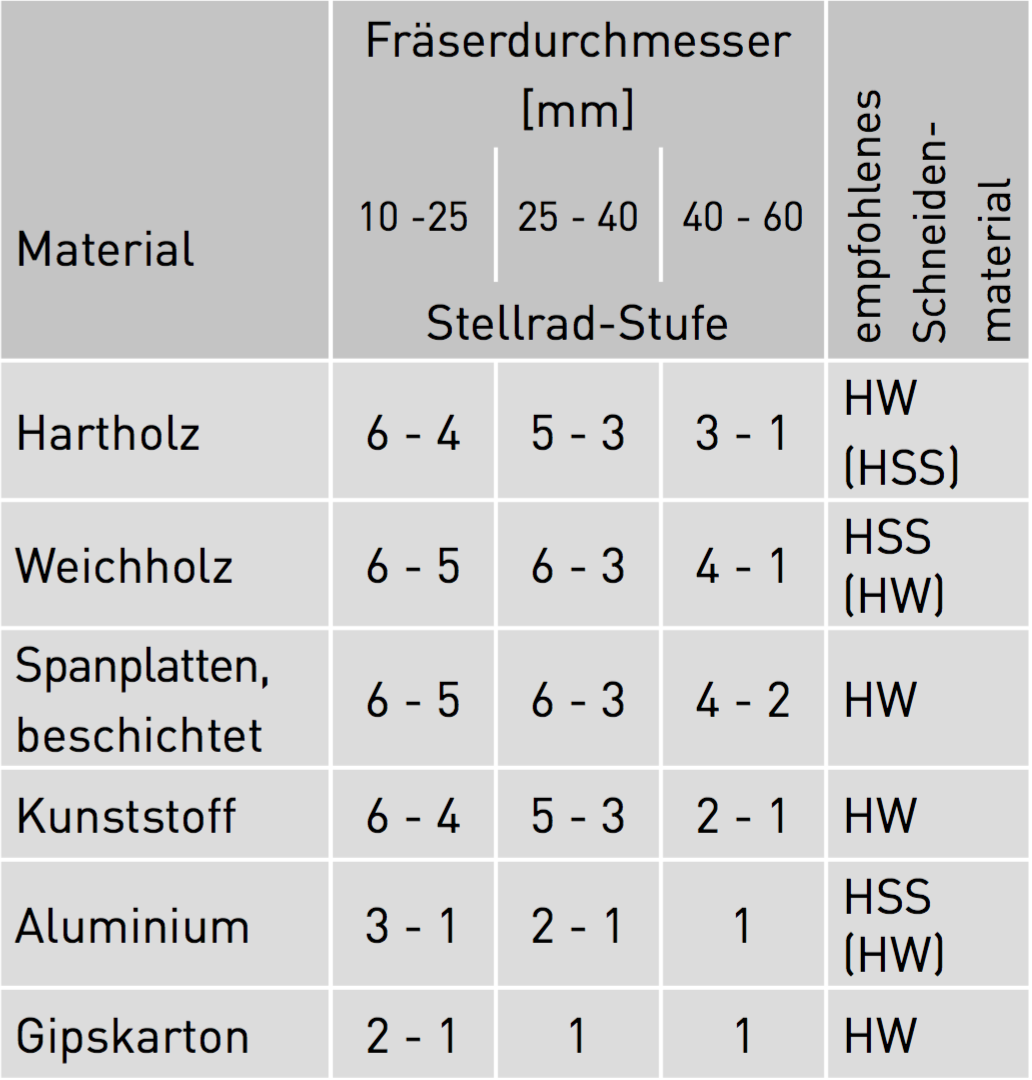
\includegraphics[width=9cm]{images/fraese_drehzahl.png}

\section{Werkstoffe}
Mit dem Standard Sägeblatt dürfen folgende Materialien bearbeitet werden:
\begin{itemize}
\item alle Holzwerkstoffe
\item Baustoffplatten
\item weiche Kunststoffe
\end{itemize}

\section{Technische Daten}
Leistungsaufnahme: 1400W\\
Leerlaufdrehzahl: 10000-22500/min\\
Max. Fräser-Ø: 60mm

\section{Einverständnisserklärung}
Einweisende/r:\\
\begin{Form}
\q{Name}
\q{Datum}
\q{Unterschrift}
\end{Form}
\leavevmode
~\\
Eingewiesene/r:\\
\begin{Form}
\q{Name}
\q{Unterschrift}
\end{Form}


\end{document}
